 %%%%%%%%%%%%%%%%%%%%%%% file template.tex %%%%%%%%%%%%%%%%%%%%%%%%%
%
% This is a general template file for the LaTeX package SVJour3
% for Springer journals.          Springer Heidelberg 2010/09/16
%
% Copy it to a new file with a new name and use it as the basis
% for your article. Delete % signs as needed.
%
% This template includes a few options for different layouts and
% content for various journals. Please consult a previous issue of
% your journal as needed.
%
%%%%%%%%%%%%%%%%%%%%%%%%%%%%%%%%%%%%%%%%%%%%%%%%%%%%%%%%%%%%%%%%%%%
%
% First comes an example EPS file -- just ignore it and
% proceed on the \documentclass line
% your LaTeX will extract the file if required
\begin{filecontents*}{example.eps}
%!PS-Adobe-3.0 EPSF-3.0
%%BoundingBox: 19 19 221 221
%%CreationDate: Mon Sep 29 1997
%%Creator: programmed by hand (JK)
%%EndComments
gsave
newpath
  20 20 moveto
  20 220 lineto
  220 220 lineto
  220 20 lineto
closepath
2 setlinewidth
gsave
  .4 setgray fill
grestore
stroke
grestore
\end{filecontents*}
%
\RequirePackage{fix-cm}
%
%\documentclass{svjour3}                     % onecolumn (standard format)
%\documentclass[smallcondensed]{svjour3}     % onecolumn (ditto)
% \documentclass[smallextended]{svjour3}       % onecolumn (second format)
\documentclass[twocolumn]{svjour3}          % twocolumn
%
\smartqed  % flush right qed marks, e.g. at end of proof
%
\usepackage{graphicx}

\usepackage{lmodern}
\usepackage{times}
%\usepackage{bm}
%\usepackage{mathptmx}
\usepackage{mathrsfs}
\usepackage[sorting=none]{biblatex}  
%\usepackage{biblatex}  
\addbibresource{ref.bib}
%\usepackage[justification=centering]{caption}
\usepackage{caption}
\usepackage{multicol}
\usepackage{caption}
\usepackage{color}
\usepackage{graphicx}
\usepackage{caption}
\usepackage{graphicx}
\usepackage{float} 

%\usepackage{subfigure}
%\usepackage{subcaption}
% \captionsetup{compatibility=false}
%\usepackage{multicolumn}
\usepackage{multirow}
\usepackage{xcolor}
\usepackage{textcomp}%
\usepackage{manyfoot}%
\usepackage{booktabs}
\usepackage{algorithm}%
\usepackage{algorithmicx}%
\usepackage{algpseudocode}%
\usepackage{listings}%
%\usepackage[number, sort&compress]{natbib}
\usepackage{cite}
\usepackage{stfloats}

\usepackage{subfig}
\usepackage{graphicx}
\usepackage{epstopdf}
\usepackage{epsfig}
\usepackage{makecell}
%\usepackage{latexsym,bm}        % 处理数学公式中和黑斜体的宏包

\usepackage{amsmath,amssymb,amsfonts}    % AMSLaTeX宏包 用来排出更加漂亮的公式
\usepackage{multirow}%
\makeatletter
\renewcommand\normalsize{%
 \@setfontsize\normalsize\@xpt\@xiipt
 \abovedisplayskip 7\p@ \@plus1\p@ \@minus6\p@
 \abovedisplayshortskip \z@ \@plus3\p@
 \belowdisplayshortskip 8\p@ \@plus3\p@ \@minus3\p@
 \belowdisplayskip \abovedisplayskip
 \let\@listi\@listI}
\makeatother


%
% \usepackage{mathptmx}      % use Times fonts if available on your TeX system
%
% insert here the call for the packages your document requires
%\usepackage{latexsym}
% etc.
%
% please place your own definitions here and don't use \def but
% \newcommand{}{}
%
% Insert the name of "your journal" with
% \journalname{myjournal}
%
\begin{document}
\begin{sloppypar}
\title{DMFF:Dual-way Multi-modal Feature Fusion for 3D Object Detection%\thanks{Grants or other notes
%about the article that should go on the front page should be
%placed here. General acknowledgments should be placed at the end of the article.}
}
% \subtitle{Do you have a subtitle?\\ If so, write it here}

%\titlerunning{Short form of title}        % if too long for running head

\author{Xiaopeng Dong         \and
        Xiaoguang Di         \and
        Wenzhuang Wang
}

%\authorrunning{Short form of author list} % if too long for running head

\institute{Xiaopeng Dong \at
              \email{596738414@qq.com}           %  \\
%             \emph{Present address:} of F. Author  %  if needed
          \and
           Xiaoguang Di(corresponding author) \at
              \email{dixiaoguang@hit.edu.cn}
          \and
           Wenzhuang Wang \at
              \email{1179828304@qq.com}
}

\date{Received: date / Accepted: date}
% The correct dates will be entered by the editor


\maketitle

\begin{abstract}
Recently, multi-modal 3D object detection that fuses the complementary information from LiDAR data and RGB images has been an active research topic. However, it is not trivial to fuse images and point clouds because of different representations of them.  Inadequate feature fusion also brings bad effects on detection performance. We convert images into pseudo point clouds by using a depth completion and utilize a more efficient feature fusion method to address the problems. In this paper, we propose a Dual-way Multi-modal Feature Fusion network (DMFF) for 3D object detection. Specifically, we first use a Dual Stream Feature Extraction module (DSFE) to generate homogeneous LiDAR and Pseudo Region of Interest (RoI) features. Then, we propose a Dual-way Feature Interaction method (DWFI) that enables inter-modal and intra-modal interaction of the two features. Next, we design a Local Attention Feature Fusion module (LAFF) to select which features of the input are more likely to contribute to the desired output. In addition, the proposed DMFF achieves the state-of-the-art performances on the KITTI Dataset.
\keywords{3D object detection\and multi-modal feature fusion\and self-attention mechanism\and Lidar point clouds\and RGB images}
% \PACS{PACS code1 \and PACS code2 \and more}
% \subclass{MSC code1 \and MSC code2 \and more}

\end{abstract}

\section{Introduction}
\label{intro}

3D object detection is a critical component of autonomous driving, where accurate results are essential for ensuring safety. Some methods based on LiDAR point clouds have been successful, such as \cite{1,2,3,4,5,6},  due to the accurate depth information they provide. However, Due to the sparsity of the point clouds, they often result in poor detection performance for long-range objects. On the other hand, RGB images lack depth information but have high resolution and rich semantic information. As a result, some multi-modal methods exploit the complementary information between LiDAR point clouds and RGB images for improving the accuracy of 3D object detection\cite{7,8,9,10}.

Currently, the most advanced fusion methods are mainly based on 3D point-cloud detectors and attempt to integrate image information into the point cloud detection process at different stages. Depending on the stage at which fusion occurs, multi-modal methods can be generally divided into three categories: early fusion, intermediate fusion and late fusion\cite{34}. Early fusion methods often enhance point clouds with image information before extracting point cloud features, which can be an effective pre-processing step to improve detection performance. However, the fusion step requires a complex 2D object detection network, leading to additional inference latency. Late fusion methods detect objects in parallel using their respective modalities, but do not utilize the deeper features of different modalities, and thus cannot integrate rich semantic information from different modalities. Intermediate fusion is more common as they fuse the rich semantic information from both modalities. There are two representative intermediate fusion methods as shown in Fig.1. The first one involves fusing features at the point/voxel level \cite{11}\cite{26}, establishing correspondences between point/voxel features and image features, enabling complementary fusion at a finer granularity.These methods usually involve combining low-level multi-scale features. However, due to the sparsity of point clouds, only partial image features can be matched. The rough correspondence between point/voxel features and image features often leads to severe information loss in this fusion method. Therefore,we adopt the other method,which is to fuse multi-modal features at the Region of Interest (RoI) \cite{12,13}. These methods typically project the 3D RoI onto a 2D plane and clip out 2D RoI features. However, due to occlusions in 2D images, the  RoI features extracted from 2D images often contain features from the background or other objects, which can interfere with the model's ability to recognize and localize the object.

\begin{figure}[h]
\centering
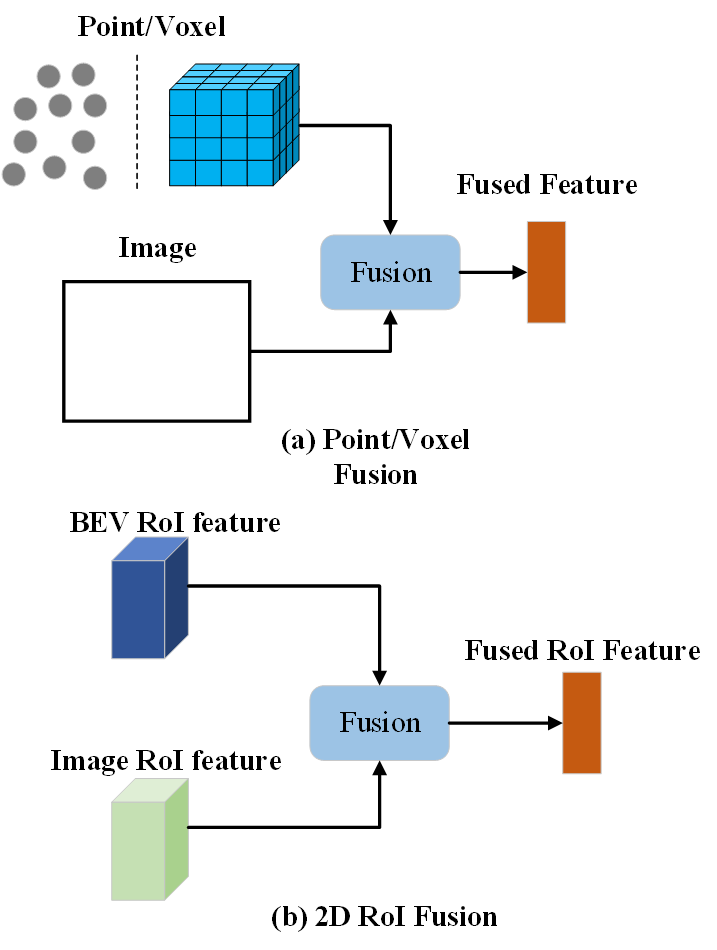
\includegraphics[width=8cm]{new_images/fig10.png}
\caption{The intermediate fusion used in previous methods.}
\label{fig_sim}
\end{figure}

To address the above issues, we propose the Dual-way Multi-modal Feature Fusion method (DMFF), which converts 2D images into 3D pseudo point clouds to avoid severe information loss caused by dimensionality reduction and to provide additional supplementary information. Specifically,when objects are occluded and contain few points, pseudo point clouds can offer ample 3D geometric information for accurate detection. Similarly, for objects located at a long distance with sparse points, the abundant points in pseudo-point clouds can provide supplementary information to precisely predict detection bounding boxes.Additionally, we represent the point clouds and pseudo point clouds using voxels and fuse their 3D RoI features at a finer granularity, thus avoiding information loss due to the mismatch between sparse point clouds and dense images. \textcolor{red}{The voxel representations of pseudo point clouds are shown in Fig.2. The generated pseudo point clouds in Fig.2 has a point density one order of magnitude higher than the original point cloud, and the pseudo point clouds have a long tail - depth artifacts around the periphery of an object stretching back into the 3D space to form a tail shape.} \textcolor{red}{
Using 3D RoI to crop pseudo point clouds in 3D space avoids occlusion issues. This is because 3D RoI contains only the features of the object of interest, while 2D RoI often include features form other objects, as shown in Fig.3.
}

\begin{figure}[h]
\centering
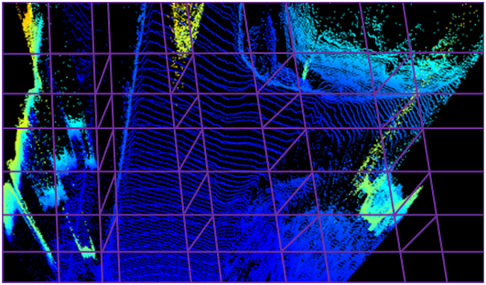
\includegraphics[width=8cm]{new_images1/fig2.png}
\captionsetup{labelfont={color=red}}
\caption{\textcolor{red}{The voxel representations of pseudo point clouds.}} 
\label{fig_sim}
\end{figure}

Specifically, the DMFF fully utilizes multi-modal information and mitigates information loss caused by inadequate fusion. DMFF consists of three core modules:(1) a dual-stream feature extraction;(2) a dual-way feature interaction; and(3) a local attention feature fusion. The dual-stream feature extraction module consists of a LiDAR stream and a Pseudo stream. LiDAR stream predict 3D RoI. Pseudo stream first gets pseudo points generated from an image by depth completion\cite{15}, and crops pseudo points using RoI, and then extracts pseudo point features. We also notice that the complementarity between the two features is extremely important. Thus, we propose the dual-way feature interaction that introduces Inter-modal Feature Interaction Module (IFIM) and Intra-modal Feature Enhancement Module (IFEM) that can achieve features interaction and enhancement. The output of the dual-way feature interaction is complementary and enhanced LiDAR RoI features and Pseudo RoI features. To further fuse features and facilitate the following detection, we utilize an attention mechanism to fuse two features. Finally, the fused RoI features are taken for further box refinement. Numerous experiments conducted on the KITTI\cite{16} Dataset show that our method can achieve better performance compared to state-of-the-art multi-modal methods.To summarize, the main contributions of our work are:

(1) We propose a dual-way feature interaction module (DWFI) that enables complete inter-modal and intra-modal information interaction among the features.

(2) We propose a dual-stream feature extraction module (DSFE) to generate homogeneous LiDAR and Pseudo RoI features. Additionally, we have utilized random resizing of 3D proposals and an auxiliary RoI head loss on the Pseudo stream to prevent the model from the over-fitting.

(3) Our method outperforms previous methods with state-of-the-art performance on KITTI 3D object detection benchmark.

%\begin{figure}[h]
%\centering
%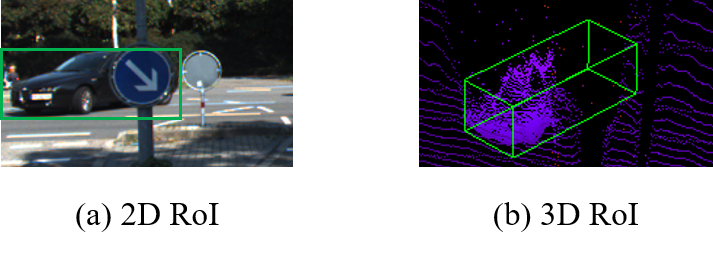
\includegraphics[width=8cm]{new_images1/RoI.png}
%\captionsetup{labelfont={color=red}}
%\caption{\textcolor{red}{The difference between 2D RoI and 3D RoI.}}
%\label{fig_sim}
%\end{figure}

\begin{figure}
        \center
        %\scriptsize
        \begin{tabular}{cc}
                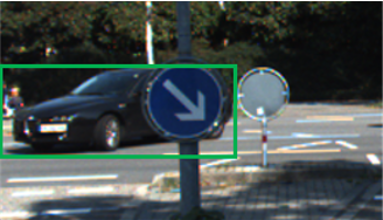
\includegraphics[width=4cm]{new_images1/2D RoI.png} &    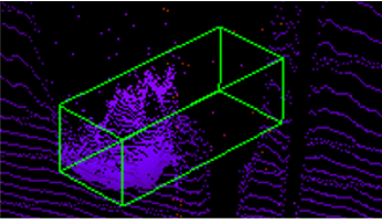
\includegraphics[width=4cm]{new_images1/3D RoI.png}         \\
                \textcolor{red}{2D RoI} & \textcolor{red}{3D RoI} \\
                
        \end{tabular}
        \captionsetup{labelfont={color=red}}
        \caption{\textcolor{red}{The difference between 2D RoI and 3D RoI.}}
        \label{figure3}
        \vspace{-0.5em}
\end{figure}

\section{Related Work}
\label{sec:1}
Nowadays,in the field of autonomous driving , the 3D object detection methods can be classified into three categories: (1) LiDAR-only 3D object detection, which utilizes the accurate range measurement of LiDAR sensors for detecting objects in 3D space; (2) Camera-only 3D object detection, which employs the rich visual information from RGB images to detect objects; (3) 3D object detection using LiDAR and camera fusion, which combines the complementary strengths of both LiDAR and camera data to achieve higher object detection accuracy.

{\bfseries 3D Object Detection Using LiDAR Only:} LiDAR-based 3D object detection methods can be divided into two streams according to the different processing methods of LiDAR point clouds: the point-based and the voxel-based. For the point-based methods, PointNet\cite{17} extracts original point cloud features using MLP and aggregates point cloud features using Max Pooling. PointNet++\cite{18} uses set abstraction to aggregate point clouds in the local region, and then exploits PointNet to extract local features. Although the point-based methods have the advantage of high object detection accuracy due to their full utilization of original point cloud information. However, the process of sampling and aggregating features from irregular point clouds is time-consuming. Additionally, these methods still have limitations in capturing the local structure information of point clouds.


Compared with time-consuming point-based methods, the voxel-based methods achieve a balance between efficiency and accuracy through sparse convolution. Voxel-based detectors discretize the disordered point cloud space into regular voxel space, thereby converting the point cloud data into voxels. VoxelNet\cite{19} extracts local features for the point clouds within each voxel using Voxel Feature Encoder(VFE). Due to the large number of empty voxels in 3D space, the 3D convolution operation in VoxelNet involves many meaningless calculations, which makes it extremely time-consuming. SECOND\cite{20} proposes 3D sparse convolution for voxels, which greatly accelerates the convolution speed. Voxel-RCNN\cite{21} utilizes the idea of two-stage detection and designs Voxel RoI pooling to aggregate local features for each proposal for further box refinement. However, voxelization introduces quantization errors in position information, resulting in geometric information loss, which affects object localization accuracy.

{\bfseries 3D Object Detection Using Camera Only:} The prevailing methods are to lift the image to the 3D space. These methods can be broadly classified into two types. The first type of methods is based on points. Pseudo-LiDAR\cite{22} uses stereo images to estimate the image depth in order to generate pseudo points. AM3D\cite{23} uses a color embedding module based on attention mechanism to enrich the features of pseudo points. 

Another type of methods is based on image features. OFT-Net\cite{24} converts image features to orthogonal BEV (Bird's Eye View) features using the Orthogonal Feature Transform module. CaDDN\cite{25} learns to generate BEV representations from images by predicting a set of depth distributions for each pixel. However, the lack of accurate depth information in monocular images results in imprecise performance of image-based methods.

{\bfseries 3D Object Detection Using Multi-modal Data:} Many multi-modal methods have been proposed to solve the problems caused by the sparsity of point clouds. Some methods fuse multi-modal data on feature level. MV3D\cite{12} and AVOD\cite{13} extract LiDAR BEV features and image features and fuse them with an RoI feature fusion strategy to make prediction. EPNet\cite{26} proposes the LI-Fusion module to fuse image features into point cloud features at different semantic levels. EPNet++\cite{27} designs IF-Fusion modules based on LI-Fusion and applies them to jointly fuse point cloud and image features.

Through explicitly projecting point clouds into 2D space and finding the corresponding image features, some works achieve the much finer granularity fusion on the point level. PointPainting\cite{28} modifies the point clouds with segmentation masks of images. PointAugmenting\cite{29} adds point clouds information by aggregating features from the middle layer of the 2D network to the corresponding point clouds. However, only a small fraction of the image information is available due to the mismatch between dense image pixels and sparse LiDAR points. 


Although many multi-modal methods have been proposed, they have not effectively fused multi-modal information. These fusion methods project 3D point clouds onto 2D planes, causing serious information loss. The coarse correspondence between the point cloud features and image features also does not fully utilize the semantic information of the images.In this paper, we generate pseudo point clouds from  images and establish accurate correspondence between point cloud features and pseudo point cloud features, achieving better 3D object detection performance.

\section{Proposed Method}
\subsection{Framework Overview}
\begin{figure}[h]
\centering
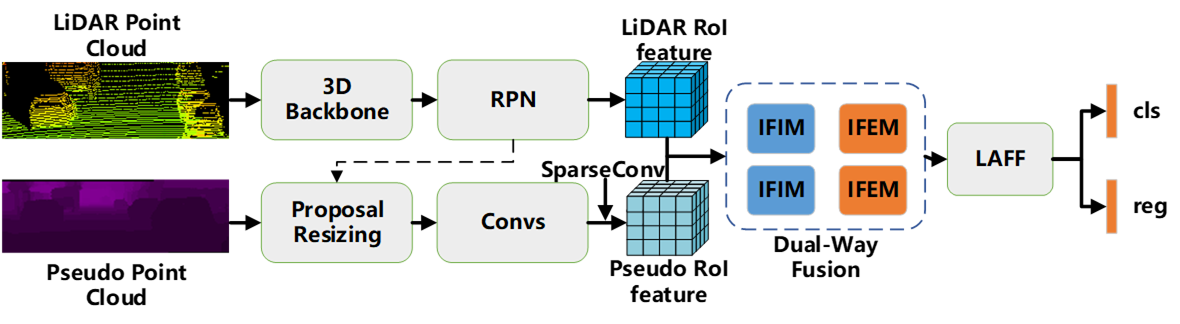
\includegraphics[width=9cm]{new_images/fig14.png}
\caption{The architecture of the proposed DMFF. Point clouds and pseudo point clouds are input to a Dual-stream Feature Extraction (DSFE) module to obtain LiDAR RoI features and Pseudo RoI features. Then, the homogeneous LiDAR and Pseudo RoI features are interacted and enhanced by dual-way feature interaction (DWFI). Last, a Local Attention Feature Fusion module (LAFF) fuses the dual-way features to produce 3D object detection results.}
\label{fig_sim}
\end{figure}

As Fig.4 illustrates, DMFF includes: (1) a two-stream feature extraction module consisting of a LiDAR branch to extract LiDAR RoI features and a Pseudo branch to extract Pseudo RoI features. (2) A dual-way feature interaction module (DWFI) that fuses 3D RoI features from two-stream structure. Each way consists of inter-modal feature interaction module (IFIM) and intra-modal feature enhancement module (IFEM). (3) A Local Attention Feature Fusion module (LAFF) further incorporates features from the DWFI.
\subsection{Dual-way Feature Interaction}
Previous methods typically used direct concatenation or a simple channel attention module to fuse two RoI features. However, they did not fully utilize the complementary information between the corresponding features, making these methods insufficient for achieving effective feature fusion.

To address the above issue, we propose the DWFI, as shown in Fig.5. It consists of two ways, each taking LiDAR Features and Pseudo Features as inputs and obtaining complementary enhanced features separately.
\begin{figure}[h]
\centering
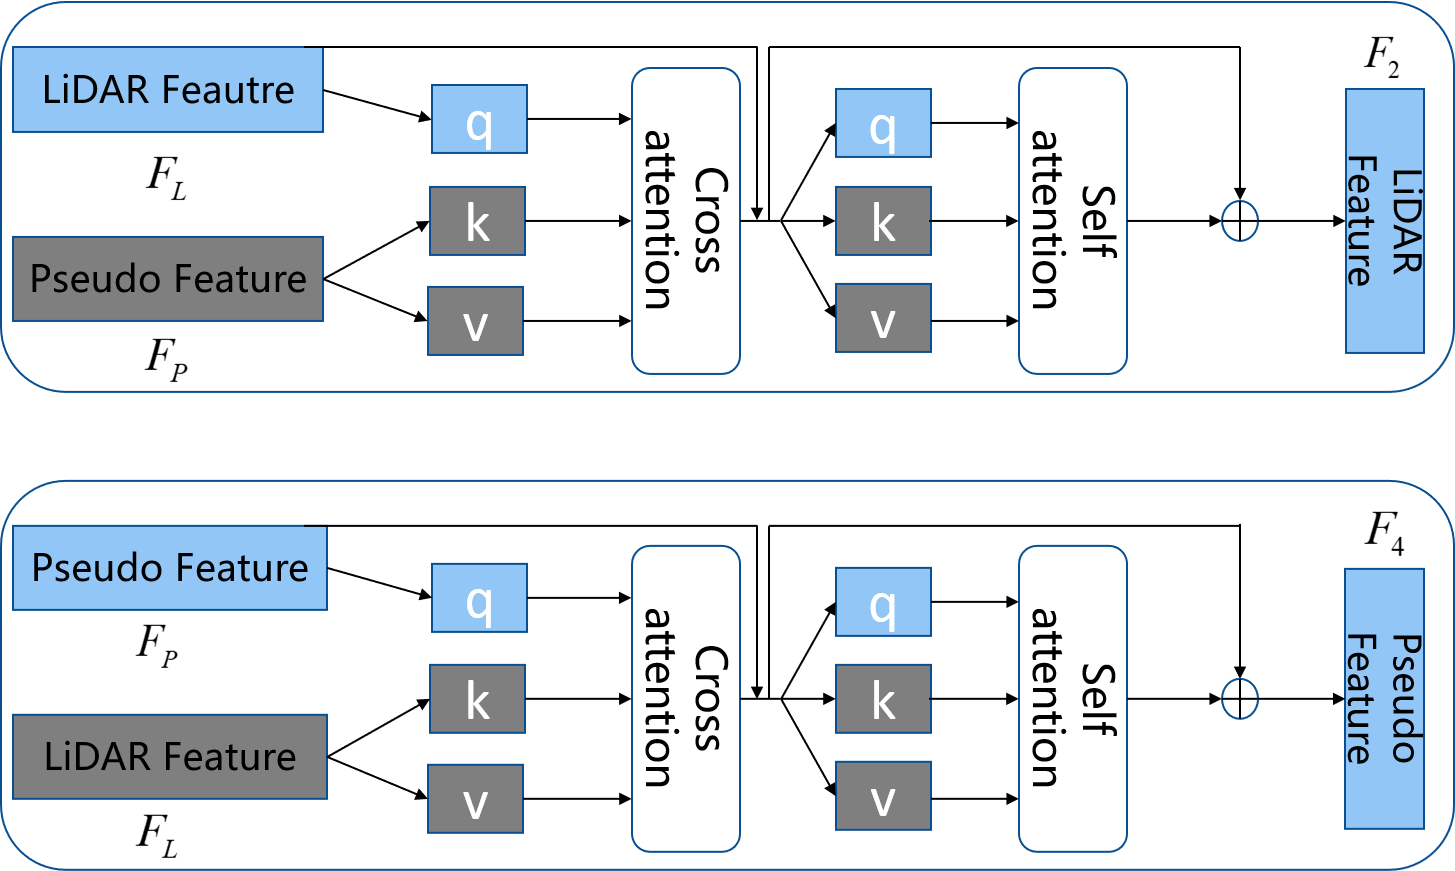
\includegraphics[width=8cm]{new_images/fig15.png}
\caption{Each way of the dual-way feature interaction consists of two parts: inter-modal feature interaction module (IFIM) and intra-modal feature enhancement module (IFEM).}
\label{fig_sim}
\end{figure}

{\bfseries IFIM.} To perform inter-modal fusion and interaction, the IFIM allows one modal features, such as LiDAR RoI features, to perceive another overall modality, such as Pseudo points converted by image, and selectively combines Pseudo RoI features. In order to efficiently aggregate complementary information between the two modalities, we propose to use a cross-attention module\cite{30}.

More specifically, we utilize the LiDAR RoI features  $F_L$ $\in$ $R^{X \times Y \times Z \times C}$ as the queries, and the Pseudo RoI features $F_P$ $\in$ $R^{X \times Y \times Z \times C}$ as the keys and the values to conduct the inter-modal fusion and form the feature $F_1$. Here ($X$,$Y$,$Z$) is the grid size following Voxel-RCNN\cite{21}, $C$ is the grid feature channel, $L$ represents the LiDAR point cloud, and $P$ represents the Pseudo point cloud.

We use a multi-head cross-attention layer as the IFIM. We apply independent learnable linear transformations on the query $F_L$, key $F_P$ and value $F_P$, the $i^{th}$ head of them are denoted as $Q_i$ $\in$ $R^{X \times Y \times Z \times d_q}$, $K_i$ $\in$ $R^{X \times Y \times Z \times d_k}$, $V_i$ $\in$ $R^{X \times Y \times Z \times d_v}$, which is described as Eqn.(1). Here, $d_q$, $d_k$, and $d_v$ represent the channel dimensions for each head.
\begin{equation}
Q_i = F_L \cdot W_{i}^{Q}, K_i = F_P \cdot W_{i}^{K}, V_i = F_P \cdot W_{i}^{V}\enspace
\end{equation}
Where $W_{i}^{Q}$ $\in$ $R^{C \times d_q}$, $W_{i}^{K}$ $\in$ $R^{C \times d_k}$, $W_{i}^{V}$ $\in$ $R^{C \times d_v}$.
Then we perform the multi-head cross-attention with $m$ heads(as shown in Eqn.(2)-(3)).
\begin{equation}
F_1 = Concat(head_1,head_2,...,head_m)+F_L\enspace
\end{equation}
\begin{equation}
head_i= {softmax}{(\frac{Q_iK_{i}^{T}}{\sqrt{d_k}})}V_i\enspace
\end{equation}
Where $F_1$ is the sum of the output from the multi-head attention module and the LiDAR RoI features $F_L$.Finally, we utilize the inter-modal fused features as the input of the IFEM module.

{\bfseries IFEM.} Compared to the IFIM which focuses on information interaction between different modalities, the IFEM emphasizes the significant information within a single modality. Specifically, we use the inter-modal fused features $F_1$ as the queries, the keys and values. Same as IFIM, we adopt a multi-head self-attention layers as IFEM, and obtain  $Q_i$ $\in$ $R^{X \times Y \times Z \times d_q}$, $K_i$ $\in$ $R^{X \times Y \times Z \times d_k}$ and $V_i$ $\in$ $R^{X \times Y \times Z \times \frac{c}{m}}$, where $Q_i$ and $K_i$ are linearly transformed.

Then we perform the multi-head self-attention with $m$ heads and add the result to $F_1$ to acquire the intra-modal fused features $F_2$.

After applying the IFIM and IFEM modules, we obtain the fused features $F_2$ from the first branch, which is a combination of LiDAR RoI features and selected Pseudo RoI features. The other branch follows a similar approach, but in this case, the Pseudo RoI features selectively combine with the LiDAR RoI features to obtain the fused features $F_4$.Formally, $F_2$ and $F_4$ are obtained by as Eqn.(4) and (5).
\begin{equation}
F_2=IFEM(IFIM(F_L,F_P))\enspace
\end{equation}
\begin{equation}
F_4=IFEM(IFIM(F_P,F_L))\enspace
\end{equation}
\subsection{Dual-Stream Feature Extraction}
We follow the similar design of MMF\cite{33} to build our backbone networks.Our inputs consist of LiDAR points obtained from LiDAR sensors and pseudo points generated from images through depth completion. The LiDAR stream gradually converts the voxelized LiDAR point clouds into feature volumes and generates 3D region proposals by employing region-proposal networks.

The points at the edges of the objects in the pseudo point clouds will extend to form a tail shape,which makes it difficult to predict the object's size. Additionally, the density of the pseudo point cloud is one order of magnitude higher than that of the original point cloud, resulting in many redundant points, which will bring unnecessary computation to the detection. Therefore, we utilize the 3D proposals to crop the pseudo points. The proposals generated from point clouds are typically quite precise, but using them directly may increase the risk of overfitting. To improve the robustness of the model, we randomly resize the 3D proposals during training.

Specifically, we randomly sample a value from a uniform distribution to add to the corresponding dimension of the 3D proposals, as shown in the Eqn.(6).
\begin{equation}
\Delta v =  \Phi{u_v},v\in{x,y,z,w,h,l,\theta} \enspace
\end{equation}
Where $\Delta v$  represents the random value in each dimension, and $\Phi$ is a uniform distribution from 0 to $u_v$, and $v$ indicates the dimensions of a bounding box, including its box center point coordinates x, y, z, box dimensions w, h, l, and the orientation angle $\theta$.

To extract rich information from the pseudo points within the 3D proposals, we utilize CPConvs\cite{14}. The extracted features are then voxelized and further processed using two sparse convolutional blocks for efficient feature extraction while maintaining high performance.

Moreover, the LiDAR stream often dominates and may lead to over-fitting. Therefore, to prevent this, we introduce an auxiliary RoI head loss on the Pseudo stream, denoted as $L_{reg2}$ . Unlike the main detection head, the auxiliary head takes the Pseudo RoI features as input and predicts the regression results of the box. By assigning different weights to the two detection heads, the loss function is defined as Eqn.(7).
\begin{equation}
L_{rcnn} = L_{IoU} + w_1*L_{reg1} + w_2*L_{reg2} \enspace
\end{equation}
Where $L_{rcnn}$ represents the loss in the proposal refinement stage, $L_{IoU}$ represents the IoU confidence prediction loss in the main detection head, $L_{reg1}$ and $L_{reg2}$ represent the 3D bounding box regression loss in the main detection head and auxiliary detection head, while $w_1$ and $w_2$ represent the loss weights of the two detection heads.

\subsection{Local Attention Feature Fusion}
To combine features from two modalities for object detection, we use an adaptive fusion network that selects the features which are most likely to contribute to the desired output. This is achieved through a attention feature fusion structure, as shown in Figure 6. The features are weighted using attention maps, which can be described as Eqn.(8)-(10).
\begin{equation}
w_1 = sigmoid(Conv_1(CONCAT(F_2,F_4))) \enspace
\end{equation}
\begin{equation}
w_2 = sigmoid(Conv_2(CONCAT(F_2,F_4))) \enspace
\end{equation}
\begin{equation}
F_{fused} = CONCAT(w_1\times F_2,w_2 \times F_4) \enspace
\end{equation}
Where $F_2$ and $F_4$ represent the LiDAR features and Pseudo features after dual-way feature interaction, $w_1$ and $w_2$ are the corresponding feature weights, respectively, $F_{fused}$ is the fused features, $\times$ is the element-wise product operation.

\begin{figure}[h]
\centering
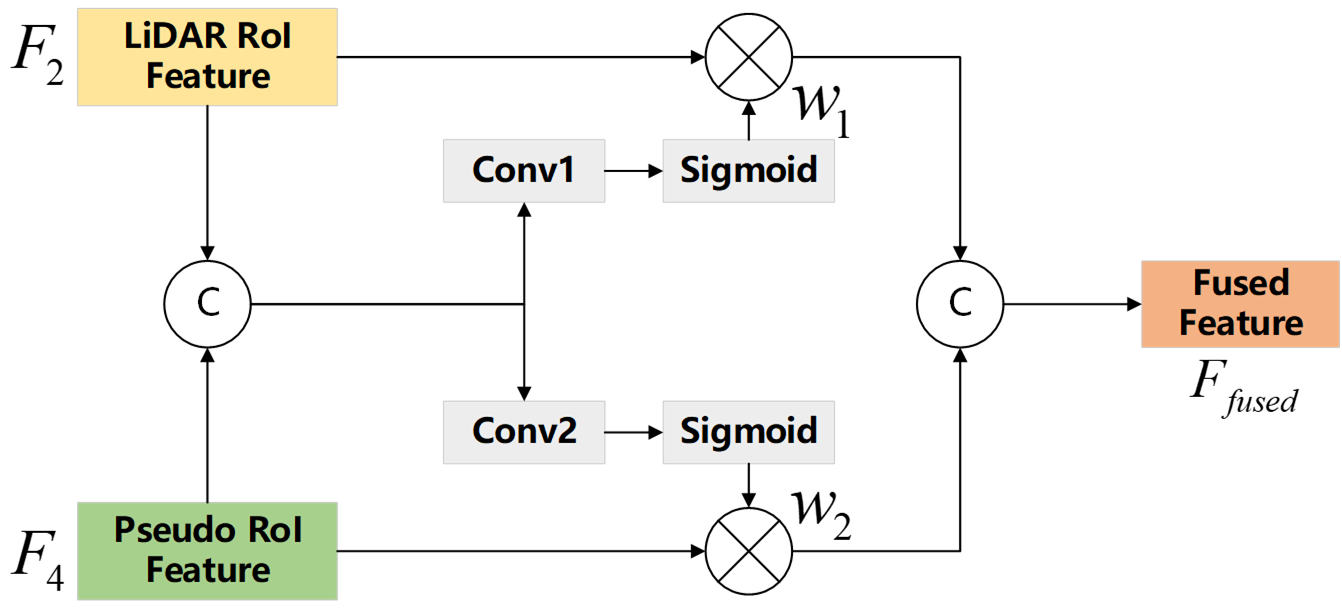
\includegraphics[width=8cm]{new_images/fig12.png}
\caption{The Local Attention Feature Fusion (LAFF) generates a pair of weights through convolution operation followed by a sigmoid function on the concatenated inputs. The inputs are weighted by the corresponding weights and then connected to obtain the fused features.}
\label{fig_sim}
\end{figure}

\subsection{Loss Function}
We implement our loss function based on Voxel-RCNN\cite{21}. The region proposal network (RPN) loss and the refinement network loss are denoted as $L_{rpn}$  and $L_{rcnn}$, respectively. The overall loss function is then defined as Eqn.(11).
\begin{equation}
L = L_{rpn} + L_{rcnn} \enspace
\end{equation}
Where $L_{rcnn}$ is defined as Eqn.(7). We adopt the same loss of RPN as in \cite{20,21}. The $L_{rpn}$ can be formulated as Eqn.(12).
\begin{equation}
L_{rpn} = a_1L_{cls} + a_2L_{reg} \enspace
\end{equation}
Where $a_1$ and $a_2$ are set to 1 and 2. We utilize the focal loss to balance the number of positive and negative samples as the classification loss, denoted as $L_{cls}$, and employ the Smooth L1 loss for the box regression.

\section{Experiments}
This section covers the dataset used to evaluate the proposed method, the experimental setup, comparison with existing state-of-the-art (SOTA) methods in dataset , and ablation experiments to validate the effectiveness of the proposed models.
\subsection{Dataset and Evaluation Metrics}
The KITTI Dataset contains 7481 samples and 7518 samples for training and testing. We divided the training data into a training set with 3712 samples and a validation set with 3769 samples. To evaluate the performance of our method, we computed the 3D object detection Average Precision ($AP_{3D}$) and the Bird's Eye View Average Precision ($AP_{BEV}$) under 40 recall thresholds (R40).

\subsection{Implementation Details}
{\bfseries Network details.} We set the range of point cloud to [0, 70.4]m, [-40, 40]m, [-3, 1]m in the (x, y, z) axis. The voxel resolution is set to (0.05, 0.05, 0.1) m. In the dual-way feature interaction, the count and hidden units of attention heads are set to 8 and 16. In the dual-stream feature extraction, we adopt the same RPN network settings as Voxel-RCNN\cite{21} and sample N = 128 proposals. Then we randomly resize the 3D proposals to crop pseudo points. The 3D proposals are rotated by [0,$\frac{2}{25}\pi$], and the rest dimensions are resized by [0m, 0.15m]. 

{\bfseries Data augmentation.}Data augmentation is a crucial approach in deep learning that can significantly improve the size and diversity of a dataset, as well as the generalization and robustness of a model.In this paper, we adopted three different data augmentation strategies, namely global rotation and flipping, local rotation and translation, and ground-truth sampling. To be more specific, the three data augmentation strategies used in our work are:(1) globally rotating the entire scene around the Z-axis with an angle sampled from a uniform distribution [$-\frac{\pi}{2}$,$\frac{\pi}{2}$] , flipping the scene along the X-axis. (2) selecting a portion of the point cloud and rotating it around a center point while translating along the coordinate axis. (3) performing the ground-truth sampling on both the point cloud and the pseudo point cloud.

\subsection{Comparison with the State-of-the-Arts methods}
{\bfseries Results on KITTI validation set.} We report the car detection results on the KITTI val set with AP calculated by 40 recall positions in Table 1. Our approach for 3D object detection achieved high average precision (AP) on the KITTI val set, with 95.66$\%$, 88.94$\%$, and 86.35$\%$ for easy, moderate, and hard levels of the car category.Our approach outperforms the other methods in terms of performance, particularly in the moderate and hard levels of the car category.Table 2 is BEV object detection AP ($\%$) on the KITTI val set. Our approach achieved 96.24$\%$ , 92.22$\%$ , and 91.88$\%$ AP in the easy, moderate, and hard levels of the car category

\begin{table*}[!t]
% increase table row spacing, adjust to taste
\renewcommand{\arraystretch}{1.3}
\setlength\tabcolsep{28pt}%调列距
\caption{Comparison with the state-of-the-art methods on the KITTI val set for car detections. The results are evaluated with the average precision of 40 sampling recall points.}
\label{table1}
\centering
% Some packages, such as MDW tools, offer better commands for making tables
% than the plain LaTeX2e tabular which is used here.
\begin{tabular*}{\linewidth}{ccccc}
\hline\noalign{\smallskip}
Methods & Modality & $AP_{3D}$(easy) & $AP_{3D}$(moderate) & $AP_{3D}$(hard) \\
% Methods & Modality & \makecell{Car \\ Easy Moderate Hard}  &  \makecell{Car \\ Easy Moderate Hard} &  \makecell{Car \\ Easy Moderate Hard} \\
\noalign{\smallskip}\hline\noalign{\smallskip}
VoxelNet\cite{19} & L & 81.97 & 65.46 & 62.85 \\
PointRCNN\cite{5} & L & 88.88 & 78.63 & 77.38 \\
PV-RCNN\cite{4} & L & 92.57 & 84.83 & 82.69 \\
Voxel-RCNN\cite{21} & L & 92.38  & 85.29 & 82.86 \\
PDV\cite{3} & L & 92.56 & 85.29 & 83.05 \\
CT3D\cite{2} & L & 92.85 & 85.82 & 83.46 \\ 
DVF-PV\cite{32} & L & 93.07 & 85.84 & 83.13 \\
MV3D\cite{12} & L+I & 71.29 & 62.68 & 56.56 \\
AVOD\cite{13} & L+I & 84.41 & 74.44 & 68.65 \\
F-PointNet\cite{10} & L+I & 83.76 & 70.92 & 63.65  \\
PointPainting\cite{11} & L+I & 88.38 & 77.74 & 76.76 \\
Focals Conv\cite{7} & L+I & 92.86 & 85.85 & 85.29 \\
Graph-VoI\cite{31} & L+I & \bf{95.67} & 86.87 & 84.09 \\
Ours &L+I & 95.66 & \bf{88.94} & \bf{86.35}\\
\noalign{\smallskip}\hline
\end{tabular*}
\end{table*}

\begin{table*}[!t]
% increase table row spacing, adjust to taste
\renewcommand{\arraystretch}{1.3}
\setlength\tabcolsep{28pt}%调列距
\caption{BEV object detection on the KITTI val set for car compared with state-of-the-art methods. The results are evaluated with the average precision of 40 sampling recall points.}
\label{table1}
\centering
% Some packages, such as MDW tools, offer better commands for making tables
% than the plain LaTeX2e tabular which is used here.
\begin{tabular*}{\linewidth}{ccccc}
\hline\noalign{\smallskip}
Methods & Modality & $AP_{3D}$(easy) & $AP_{3D}$(moderate) & $AP_{3D}$(hard) \\
\noalign{\smallskip}\hline\noalign{\smallskip}
VoxelNet\cite{19} & L & 77.47 & 65.11 & 57.73\\
PV-RCNN\cite{4} & L & 95.76 & 91.11 & 88.93 \\
Voxel-RCNN\cite{21} & L & 95.52  & 91.25 & 88.99 \\
CT3D\cite{2} & L & 96.14 & 91.88 & 89.63 \\
DVF-PV\cite{32} & L & 96.21 & 91.66 & 89.17 \\
MV3D\cite{12} & L+I & 86.02 & 76.90 & 68.49 \\
AVOD\cite{13} & L+I & 86.80 & 85.44 & 77.73 \\
F-PointNet\cite{10} & L+I & 88.70 & 84.00 & 75.33 \\
Ours &L+I & \bf{96.24} & \bf{92.22} & \bf{91.88}\\
\noalign{\smallskip}\hline
\end{tabular*}
\end{table*}


\subsection{Ablation Studies}
In this section, we conduct an ablation study on the KITTI validation set to evaluate the impact of each component in our proposed method. 
\subsubsection{Effect of Dual-way Feature Interaction.}
The dual-way feature interaction (DWFI) plays a key role in our proposed multi-modal detection framework by allowing the two types of features to complement each other and obtain the enhanced features. Through the DWFI, our approach can effectively exploit the strengths of LiDAR point cloud and pseudo point cloud data, leading to better feature representation for accurate 3D object detection. In Table 3, ‘w/o DWFI’ represent  ‘without DWFI’. We observe that DWFI can lead to 0.15 $\%$, 0.33 $\%$, and 0.54 $\%$ performance improvement in $AP_{Easy}$,  $AP_{Mod}$, $AP_{Hard}$. We have observed that the dual-way feature interaction is particularly efficient for heavily-occluded object detections in the hard category.
\subsubsection{Effect of Proposal Random Resizing.}
Here, we remove the random resizing component to evaluate its impact, as shown in Table 3. We find that the proposal random resizing can bring 0.05 $\%$, 0.15 $\%$, 0.34 $\%$, performance gains in
 $AP_{Easy}$,  $AP_{Mod}$, $AP_{Hard}$.  \textcolor{red}{ By expanding the size of the proposal, more contextual information can be included. Randomly enlarging the size allows the network to determine which information is necessary.}
 \subsubsection{Effect of Local Attention Feature Fusion.}
 We replaced local attention feature fusion with channel concatenation operation. We observe that the local attention feature fusion can bring 0.2 $\%$, 0.31 $\%$, and 0.41 $\%$ performance gains in $AP_{Easy}$,  $AP_{Mod}$, $AP_{Hard}$. This suggests that the LAFF is a crucial and effective module in our multi-modal detection framework. \textcolor{red}{By selectively combining those LiDAR and Pseudo features that are most likely to contribute to the desired output, our method can generate the enhanced fused features.}

 \begin{table}[!t]
% increase table row spacing, adjust to taste
\renewcommand{\arraystretch}{1.3}
\setlength\tabcolsep{15pt}%调列距
\caption{The ablation studies to evaluate the impact of our proposed modules.}
\label{table3}
\centering
% Some packages, such as MDW tools, offer better commands for making tables
% than the plain LaTeX2e tabular which is used here.
\begin{tabular}{cccc}
\hline\noalign{\smallskip}
Methods & 3D Easy & 3D Mod & 3D Hard \\
\noalign{\smallskip}\hline\noalign{\smallskip}
DMFF & 95.66 & 88.94 & 86.35 \\
w/o DWFI & 95.51 & 88.61 & 85.81 \\
w/o PRR & 95.61 & 88.79 & 86.01\\
w/o LAFF & 95.46 & 88.63 & 85.94 \\
\noalign{\smallskip}\hline
\end{tabular}
\end{table}

\subsection{Qualitative Results}
We have also included some qualitative visualization results in Figure 7 to demonstrate the effectiveness of our approach. Our method is capable of accurately detecting objects in diverse scenes, including those with occlusions and objects located at far distances. Our approach has shown reliable performance in detecting objects in complex real world.

\subsection{{Inference Speed}}
\textcolor{red}{We test the inference speed of our DMFF on an NVIDIA RTX 2080 Ti GPU. The runtime of our method was measured at 95ms, with approximately 40ms dedicated to generating a comprehensive pseudo-point cloud. While it is true that DMFF, being a multi-modal detector, might be comparably slower than certain single-modal methods. However, in multi-modal methods, DMFF inference speed is competitive, as shown in Table 4.}


\subsection{{Multi-class object detection performance}}
\textcolor{red}{We also trained a multi-class DMFF model capable of detecting instances from car, pedestrian, and cyclist classes using a single unified model. We reported the multi-class 3D object detection performance in Table 5. When compared with other
SOTA methods that provide multi-class object detection results, the detection performance of DMFF has been significantly improved in all classes. The results demonstrate that our DMFF can be easily generalized to a multi-class model, effectively enhancing detection performance.}

 \begin{table}[!t]
% increase table row spacing, adjust to taste
\renewcommand{\arraystretch}{1.3}
\setlength\tabcolsep{9pt}%调列距
\captionsetup{labelfont={color=red}}
\caption{\textcolor{red}{Inference speed of different multi-modal methods.}}
\label{table4}
\centering
% Some packages, such as MDW tools, offer better commands for making tables
% than the plain LaTeX2e tabular which is used here.
\begin{tabular}{cccc}
\hline\noalign{\smallskip}
\color{red}{Ours} & \color{red}{AVOD\cite{13}} & \color{red}{F-PointNet\cite{10}} & \color{red}{Focals Conv\cite{7}} \\
\noalign{\smallskip}\hline\noalign{\smallskip}
\color{red}{95ms} & \color{red}{80ms} & \color{red}{170ms} & \color{red}{100ms} \\
\noalign{\smallskip}\hline
\end{tabular}
\end{table}

 \begin{table}[!t]
% increase table row spacing, adjust to taste
\renewcommand{\arraystretch}{1.3}
\setlength\tabcolsep{8pt}%调列距
\captionsetup{labelfont={color=red}}
\caption{\textcolor{red}{Performance of DMFF on the KITTI val set for car, pedestrian and cyclist with AP calculated by 40 recall positions.}}
\label{table5}
\centering
% Some packages, such as MDW tools, offer better commands for making tables
% than the plain LaTeX2e tabular which is used here.
\begin{tabular}{ccccc}
\hline\noalign{\smallskip}
\multirow{2}{*}{\color{red}{Class}} & \multirow{2}{*}{\color{red}{Method}} & ~ & \color{red}{3D AP} \\
~ & ~ & \color{red}{Easy} & \color{red}{Mod} & \color{red}{Hard} \\
\noalign{\smallskip}\hline\noalign{\smallskip}
\color{red}{Car} & \makecell{\color{red}{DVF-PV\cite{32}} \\ \color{red}{Focals Conv\cite{7}} \\ \color{red}{DMFF} } & \makecell{\color{red}{92.45} \\ \color{red}{92.32} \\ \color{red}{95.51}} & \makecell{\color{red}{85.28} \\ \color{red}{85.19} \\ \color{red}{88.62}} & \makecell{\color{red}{82.84} \\ \color{red}{82.62} \\ \color{red}{86.39}} \\
\noalign{\smallskip}\hline
\color{red}{Pedestrian} & \makecell{\color{red}{DVF-PV\cite{32}} \\ \color{red}{Focals Conv\cite{7}} \\ \color{red}{DMFF}} & \makecell{\color{red}{70.13} \\ \color{red}{N/A} \\ \color{red}{73.11}} & \makecell{\color{red}{62.76} \\ \color{red}{61.61} \\ \color{red}{66.78}} & \makecell{\color{red}{57.65} \\ \color{red}{N/A} \\ \color{red}{60.79}} \\
\noalign{\smallskip}\hline
\color{red}{Cyclist} & \makecell{\color{red}{DVF-PV\cite{32}} \\ \color{red}{Focals Conv\cite{7}} \\ \color{red}{DMFF}} & \makecell{\color{red}{90.93} \\ \color{red}{N/A} \\ \color{red}{91.32}} & \makecell{\color{red}{72.60} \\ \color{red}{72.76} \\ \color{red}{73.26}} & \makecell{\color{red}{68.24} \\ \color{red}{N/A} \\ \color{red}{67.95}} \\
\hline\noalign{\smallskip}
\end{tabular}
\end{table}

\begin{figure*}
        \center
        \scriptsize
        \begin{tabular}{cc}
                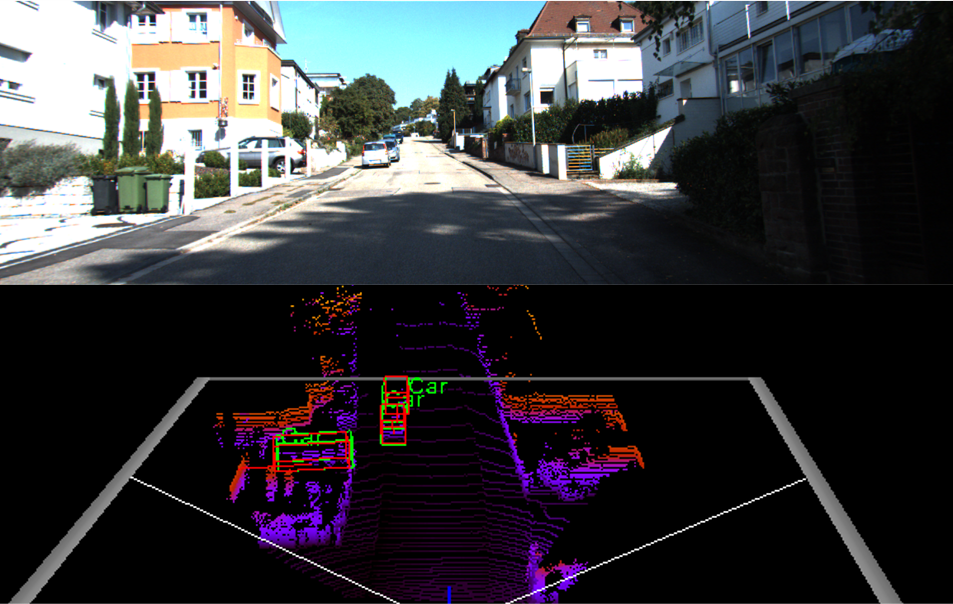
\includegraphics[width=8cm]{./kitti/1.png} &
                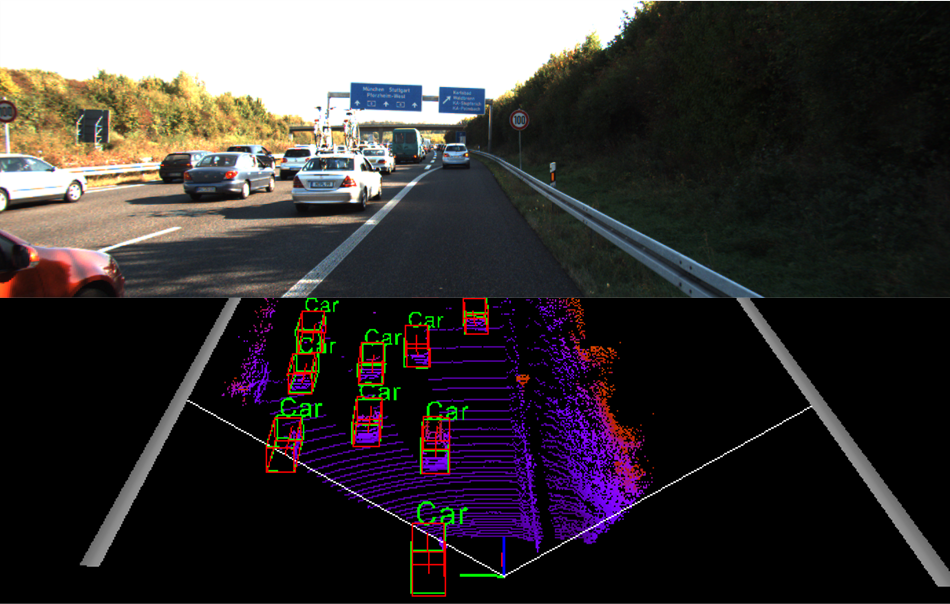
\includegraphics[width=8cm]{./kitti/2.png} \\
                
                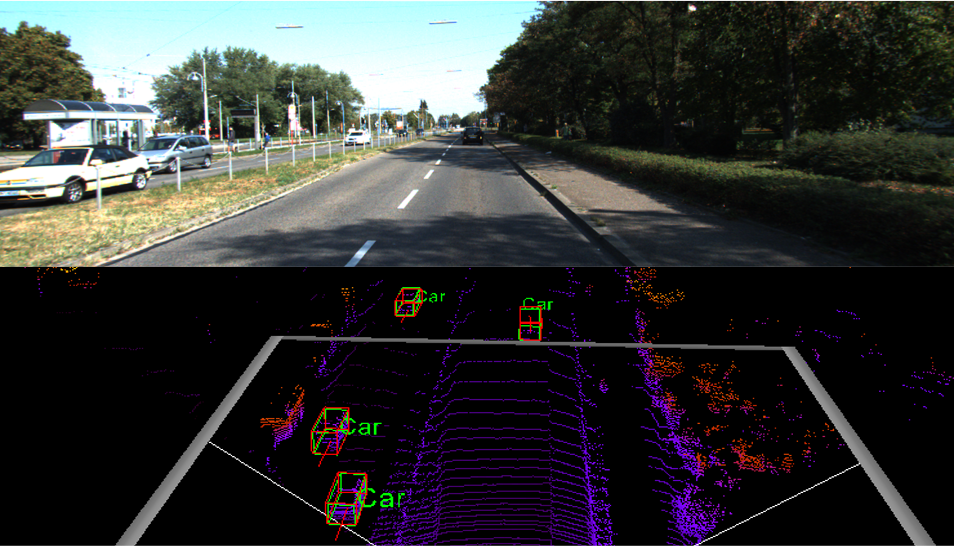
\includegraphics[width=8cm]{./kitti/3.png}  &  
                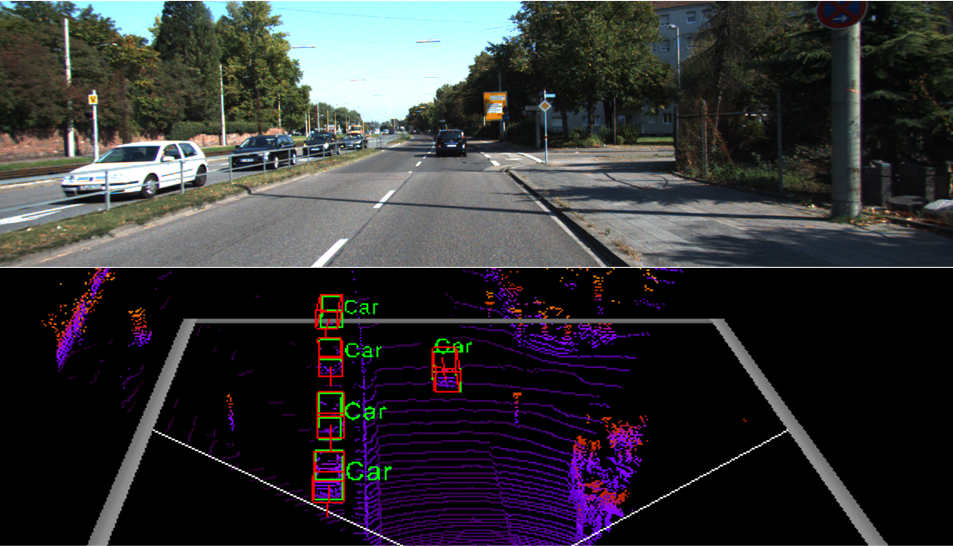
\includegraphics[width=8cm]{./kitti/4.png}  \\
        \end{tabular}
        \caption{\textcolor{black}{Qualitative results of our method on KITTI. From top to bottom, each pair of images consists of a 2D image and its corresponding 3D detection result. The green box on the 3D detection result marks the ground truth box, while the red box marks the prediction box. }}
        \label{figure10}
        \vspace{-0.5em}
\end{figure*}

\section{Conclusion}
In this paper, we propose the Dual-way Multi-modal Features Fusion for 3D object Detection (DMFF). Our approach utilizes a dual-way feature fusion to enable full inter-modal information complementarity and intra-modal information enhancement among the features. The use of dual-stream feature extraction helps to create homogenous pseudo RoI features with LiDAR RoI features. Moreover, we propose a local attention feature fusion to determine which input features are more likely to contribute to the desired output. Our experiments on the KITTI dataset demonstrate significant improvements in detection accuracy compared with other SOTA methods.


% Authors must disclose all relationships or interests that 
% could have direct or potential influence or impart bias on 
% the work: 
%
% \section*{Conflict of interest}
%
% The authors declare that they have no conflict of interest.


% BibTeX users please use one of
%\bibliographystyle{spbasic}      % basic style, author-year citations
%\bibliographystyle{spmpsci}      % mathematics and physical sciences
%\bibliographystyle{spphys}       % APS-like style for physics
%\bibliography{}   % name your BibTeX data base

% Non-BibTeX users please use
% \begin{thebibliography}{}
% %
% % and use \bibitem to create references. Consult the Instructions
% % for authors for reference list style.
% %
% \bibitem{RefJ}
% % Format for Journal Reference
% Author, Article title, Journal, Volume, page numbers (year)
% % Format for books
% \bibitem{RefB}
% Author, Book title, page numbers. Publisher, place (year)
% etc
% \end{thebibliography}


%\bibliographystyle{spphys}
%\bibliographystyle{unsrt}
\begin{thebibliography}{33}
	\bibitem{1}Zhou, C., Zhang, Y., Chen, J., and Huang, D.: OcTr: Octree-based Transformer for 3D Object Detection. arXiv preprint arXiv:2303.12621 (2023)
	\bibitem{2}Sheng, H., Cai, S., Liu, Y., Deng, B., Huang, J., Hua, X. S., Zhao, M. J.: Improving 3d object detection with channel-wise transformer. In: Proceedings of the IEEE/CVF Conference on Computer Vision and Pattern Recognition. pp. 2743-2752 (2021)
	\bibitem{3}Hu, J. S., Kuai, T., and Waslander, S. L.: Point density-aware voxels for lidar 3d object detection. In: Proceedings of the IEEE/CVF Conference on Computer Vision and Pattern Recognition. pp. 8469-8478 (2022)
	\bibitem{4}Shi, S., Guo, C., Jiang, L., Wang, Z., Shi, J., Wang, X., Li, H.: Pv-rcnn: Point-voxel feature set abstraction for 3d object detection. In: CVPR. pp. 10529–10538 (2020)
	\bibitem{5}Shi, S., Wang, X., Li, H.: Pointrcnn: 3d object proposal generation and detection from point cloud. In: CVPR. pp. 770–779 (2019)	
	\bibitem{6}Xu, Q., Zhong, Y., and Neumann, U.: Behind the curtain: Learning occluded shapes for 3d object detection. In: Proceedings of the AAAI Conference on Artificial Intelligence. pp. 2893-2901 (2022)
	\bibitem{7}Chen, Y., Li, Y., Zhang, X., Sun, J., and Jia, J.: Focal sparse convolutional networks for 3d object detection. In: Proceedings of the IEEE/CVF Conference on Computer Vision and Pattern Recognition. pp. 5428-5437 (2022)
	\bibitem{8}Zhu, H., Deng, J., Zhang, Y., Ji, J., Mao, Q., Li, H., and Zhang, Y.: Vpfnet: Improving 3d object detection with virtual point based lidar and stereo data fusion. arXiv preprint arXiv:2111.14382 (2021)
	\bibitem{9}Liu, Z., Tang, H., Amini, A., Yang, X., Mao, H., Rus, D., and Han, S.: BEVFusion: Multi-Task Multi-Sensor Fusion with Unified Bird's-Eye View Representation. arXiv preprint arXiv:2205.13542 (2022)
        \bibitem{10}Qi, C.R., Liu, W., Wu, C., Su, H., Guibas, L.J.: Frustum 
    pointnets for 3d object detection from rgb-d data. In: CVPR. pp. 918–927 (2018)
        \bibitem{11}Vora, S., Lang, A.H., Helou, B., Beijbom, O.: Pointpainting: 
    Sequential fusion for 3d object detection. In: CVPR. pp. 4604–4612 (2020)
        \bibitem{12}Chen, X., Ma, H., Wan, J., Li, B., Xia, T.: Multi-view 3d 
    object detection network for autonomous driving. In: CVPR. pp. 1907–1915 (2017)
        \bibitem{13}Ku, J., Mozifian, M., Lee, J., Harakeh, A., Waslander, S.L.: 
    Joint 3d proposal generation and object detection from view aggregation. In: IEEE/RSJ International Conference on Intelligent Robots and Systems (IROS). pp. 1–8. IEEE (2018)
        \bibitem{14}Wu, X., Peng, L., Yang, H., Xie, L., Huang, C., Deng, C., ... 
    and Cai, D.: Sparse fuse dense: Towards high quality 3d detection with depth completion. In: Proceedings of the IEEE/CVF Conference on Computer Vision and Pattern Recognition. pp. 5418-5427 (2022)
        \bibitem{15}Hu, M., Wang, S., Li, B., Ning, S., Fan, L., and Gong, X.: 
    Penet: Towards precise and efficient image guided depth completion. In 2021 IEEE International Conference on Robotics and Automation (ICRA). pp. 13656-13662. IEEE (2021)
        \bibitem{16}Geiger, A., Lenz, P., Urtasun, R.: Are we ready for 
    autonomous driving? the kitti vision benchmark suite. In: CVPR. pp. 3354–3361 (2012)
        \bibitem{17}Qi, C.R., Su, H., Mo, K., Guibas, L.J.: Pointnet: Deep 
    learning on point sets for 3d classification and segmentation. In: CVPR. pp. 652–660 (2017)
        \bibitem{18}Qi, C.R., Yi, L., Su, H., Guibas, L.J.: Pointnet++: Deep 
    hierarchical feature learning on point sets in a metric space. NeurIPS 30 (2017)
        \bibitem{19}Zhou, Y., Tuzel, O.: Voxelnet: End-to-end learning for point 
    cloud based 3d object detection. In: CVPR. pp. 4490–4499 (2018)
	\bibitem{20}Yan, Y., Mao, Y., Li, B.: Second: Sparsely embedded convolutional detection. Sensors 18(10), 3337 (2018)
	\bibitem{21}Deng, J., Shi, S., Li, P., Zhou, W., Zhang, Y., Li, H.: Voxel r-cnn: Towards high performance voxel-based 3d object detection. In: AAAI. pp. 1201–1209 (2021)
	\bibitem{22}Wang, Y., Chao, W. L., Garg, D., Hariharan, B., Campbell, M., and Weinberger, K. Q.: Pseudo-lidar from visual depth estimation: Bridging the gap in 3d object detection for autonomous driving. In: Proceedings of the IEEE/CVF Conference on Computer Vision and Pattern Recognition. pp. 8445-8453 (2019)
	\bibitem{23}Ma, X., Wang, Z., Li, H., Zhang, P., Ouyang, W., and Fan, X.: Accurate monocular 3d object detection via color-embedded 3d reconstruction for autonomous driving. In: Proceedings of the IEEE/CVF International Conference on Computer Vision. pp. 6851-6860 (2019)
	\bibitem{24}Roddick, T., Kendall, A., and Cipolla, R.: Orthographic feature transform for monocular 3d object detection. arXiv preprint arXiv:1811.08188 (2018)
	\bibitem{25}Reading, C., Harakeh, A., Chae, J., Waslander, S.L.: Categorical depth distribution network for monocular 3d object detection. In: CVPR. pp. 8555–8564 (2021)
	\bibitem{26}Huang, T., Liu, Z., Chen, X., Bai, X.: Epnet: Enhancing point features with image semantics for 3d object detection. In: ECCV. pp. 35–52. Springer (2020)
	\bibitem{27}Liu, Z., Huang, T., Li, B., Chen, X., Wang, X., and Bai, X.: EPNet++: Cascade bi-directional fusion for multi-modal 3D object detection. arXiv preprint arXiv:2112.11088 (2021)
        \bibitem{28}Vora, S., Lang, A.H., Helou, B., Beijbom, O.: Pointpainting: 
    Sequential fusion for 3d object detection. In: CVPR. pp. 4604–4612 (2020)
        \bibitem{29}Wang, C., Ma, C., Zhu, M., Yang, X.: Pointaugmenting: Cross-
    modal augmentation for 3d object detection. In: CVPR. pp. 11794–11803 (2021)
        \bibitem{30}Vaswani, A., Shazeer, N., Parmar, N., Uszkoreit, J., Jones, 
    L., Gomez, A. N., ... and Polosukhin, I.: Attention is all you need. Advances in neural information processing systems, 30 (2017)
        \bibitem{31}Yang, H., Liu, Z., Wu, X., Wang, W., Qian, W., He, X., and 
    Cai, D.: Graph R-CNN: Towards Accurate 3D Object Detection with Semantic-Decorated Local Graph. In: ECCV. pp. 662-679. Springer (2022)
        \bibitem{32}Mahmoud, A., Hu, J. S., and Waslander, S. L.: Dense voxel 
    fusion for 3D object detection. In: Proceedings of the IEEE/CVF Winter Conference on Applications of Computer Vision. pp. 663-672 (2023)
        \bibitem{33}Liang, M., Yang, B., Chen, Y., Hu, R., and Urtasun, R.: Multi-
    task multi-sensor fusion for 3d object detection. In: Proceedings of the IEEE/CVF Conference on Computer Vision and Pattern Recognition. pp. 7345-7353 (2019)
        \bibitem{34}Wang, Y., Mao, Q., Zhu, H., Deng, J., Zhang, Y., Ji, J., ... and Zhang, Y.: Multi-modal 3d object detection in autonomous driving: a survey. arXiv preprint arXiv:2106.12735 (2021)

       
    
\end{thebibliography}

\def\bibfont{\fontsize{10.5}\selectfont}
% \bibliography{ref}
%\printbibliography
%\iffalse

\twocolumn[
\begin{@twocolumnfalse}
\section*{\centering{\huge Declarations}}

\renewcommand{\labelitemi}{\textbullet}


\begin{itemize}

\setlength{\itemsep}{5pt}

\setlength{\parsep}{5pt}

\setlength{\parskip}{5pt}
\large \item \textbf{Ethics approval and consent to participate}

Not applicable

\item \textbf{Consent for publication}

Not applicable

\item \textbf{Availability of data and materials}

Not applicable

\item \textbf{Competing interests}

The authors declare that they have no competing interests.

\item \textbf{Funding}

This work was supported in part by the Natural Science Foundation of
Heilongjiang Province of China (No.LH2021F026), Fundamental Research Funds for the Central Universities(No. HIT.NSRIF202243) and Aeronautical Science Foundation of China(No.2022Z071077002).


\item \textbf{Authors' contributions}

Xiaopeng Dong and Xiaoguang Di designed the research. Xiaopeng Dong drafted the manuscript. Xiaoguang Di helped organize the manuscript. 

\item \textbf{Acknowledgements}

We appreciated the Natural Science Foundation of Heilongjiang Province of China (No.LH2021F026), Fundamental Research Funds for the Central
Universities(No. HIT.NSRIF202243) and Aeronautical Science Foundation of China(No.2022Z071077002) for their support.

\item \textbf{Authors' information (optional)}

\textbf{Xiaopeng Dong} received the B.S. degree in automation from Hefei University of Technology, China, in 2021. He is currently a graduate student at the Control and Simulation Center, Harbin Institute of Technology. His current research interests include deep learning and 3D object detection.

\textbf{Xiaoguang Di} (corresponding author) is currently a Professor with the Control and Simulation Center, Harbin Institute of Technology. His current research interests include image restoration and enhancement, object detection and recognition, deep learning, and SLAM. He is a member of the Chinese Association of Automation and the China Simulation Federation.

\textbf{Wenzhuang Wang} is currently working toward the M.S. in the School of Astronautics, Harbin Institute of Technology. His research interests include multimodal learning, remote sensing object detection, and deep learning.



\end{itemize}
\end{@twocolumnfalse}
]
%\fi

\clearpage


\end{sloppypar}
%\bibliographystyle{spphys}
%\bibliography{ref}
\end{document}
% end of file template.tex

